\documentclass{standalone}
\usepackage{tikz}
\usepackage{ctex,siunitx}
\setCJKmainfont{Noto Serif CJK SC}
\usepackage{tkz-euclide}
\usepackage{amsmath}
\usepackage{wasysym}
\usetikzlibrary{patterns, calc}
\usetikzlibrary {decorations.pathmorphing, decorations.pathreplacing, decorations.shapes,}
\begin{document}
\small
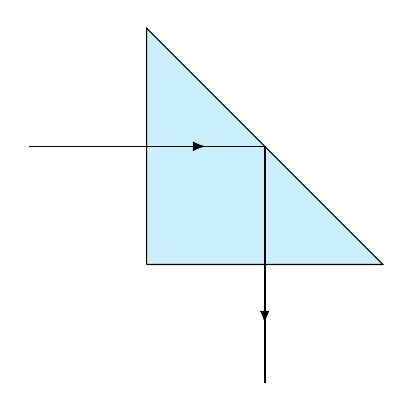
\begin{tikzpicture}[>=latex,scale=1.5]
  \draw [fill=cyan!20](0,0)--(2,0)--(0,2)--(0,0);
  \draw[semithick] (-1,1)--(1,1)--(1,-1);
  \draw[->,semithick](-1,1)--(.5,1); 
  \draw[->,semithick](1,1)--(1,-.5); 
\end{tikzpicture}
\end{document}